%----------------------------------------------------------------------------
\chapter{\bevezetes}
%----------------------------------------------------------------------------

\section{Motivation}

Nowadays mobile robots' navigation is researched worldwide. If we think about it, it is essential for these autonomous vehicles to thoroughly explore their surroundings before starting their tasks. It is not advised for any of them to go wandering in their environment because they will get lost.

One of the simplest examples is a robot vacuum cleaner. To make things more exciting I can provide some firsthand experiences because I own an iRobot Roomba 780 and my parents own an iRobot Roomba i7. The 780 is an older model from 2010, it just wanders from wall to wall in the house, it does not use any localization or mapping at all. On the other hand, the i7 has a camera on top of it which can see the ceiling of the rooms. At the first run it executes a mapping sequence, so it just goes around the rooms without "thinking". After the mapping has finished we can see the mapped rooms on the app. The i7 is much more flexible because it knows where is its docking station and it can fully localize itself in the rooms so it can vacuum systematically. On the contrary, the 780 just goes around, from wall to wall, hectically like a lunatic.

\begin{figure}[H]
	\centering
	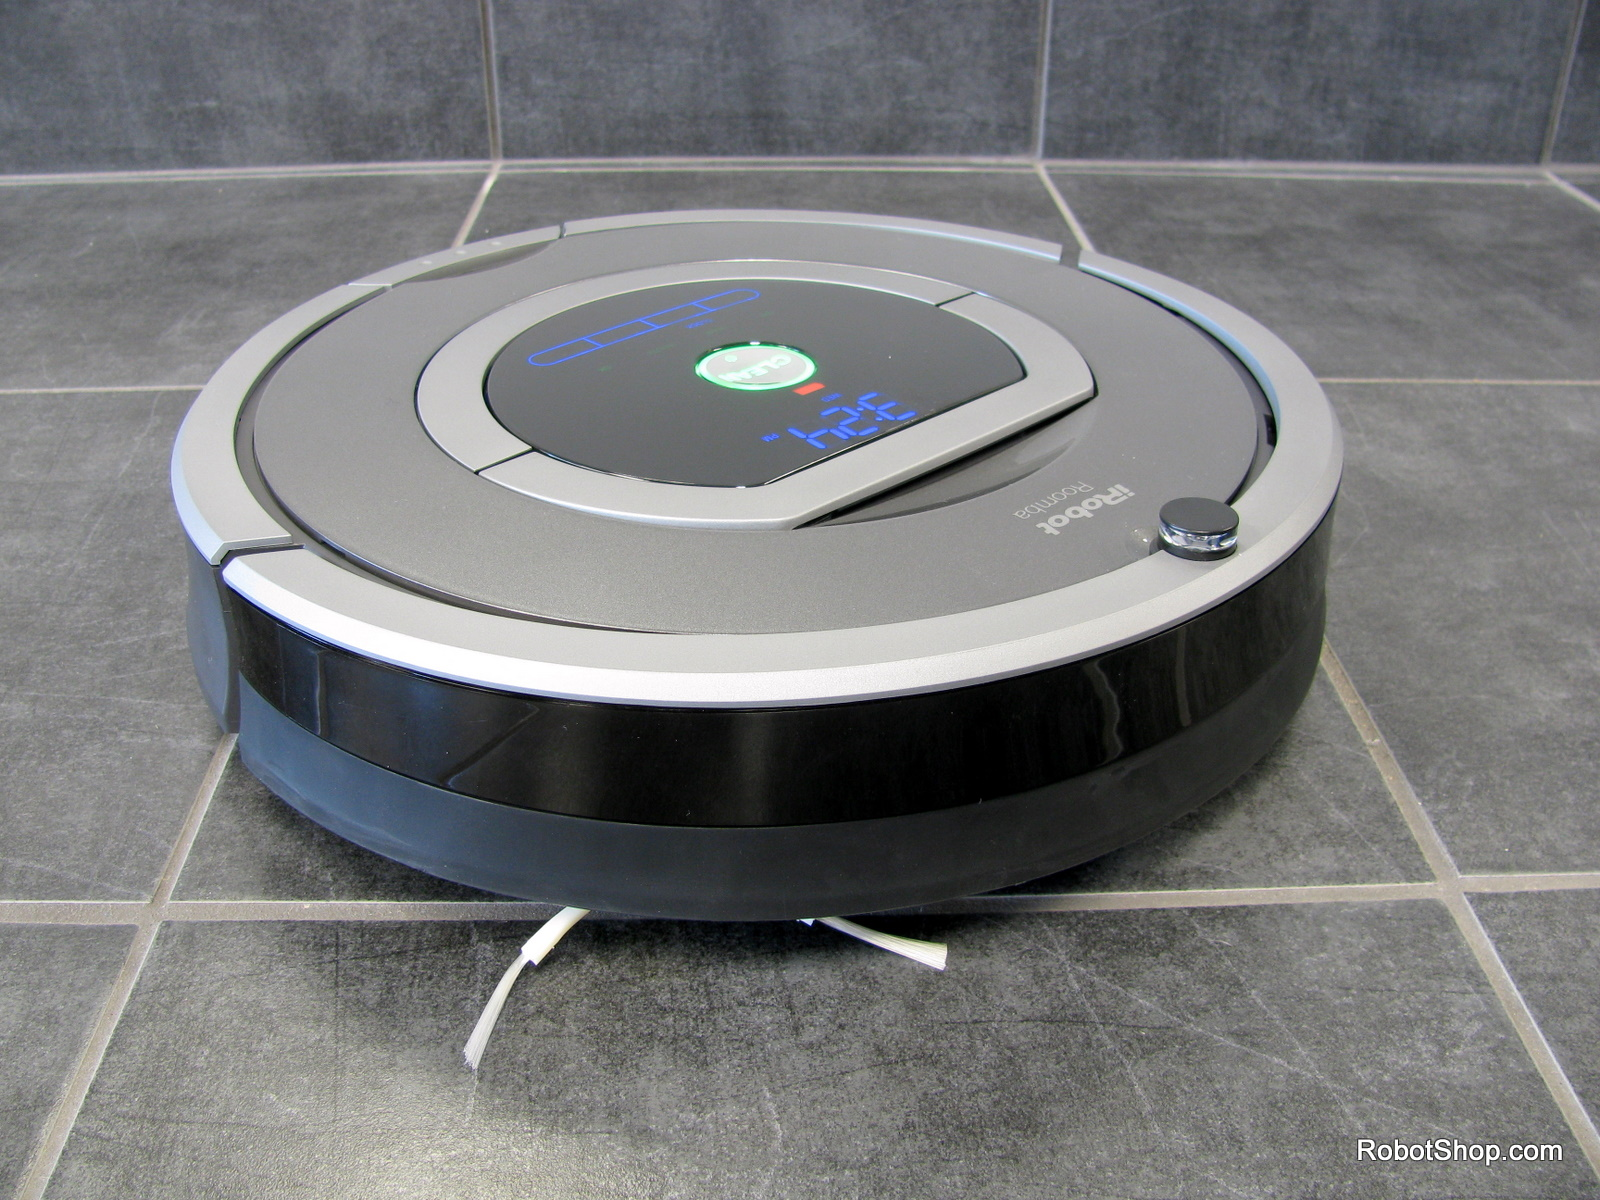
\includegraphics[width=67mm, keepaspectratio]{figures/iRobot_roomba_780.jpg}\hspace{1cm}
	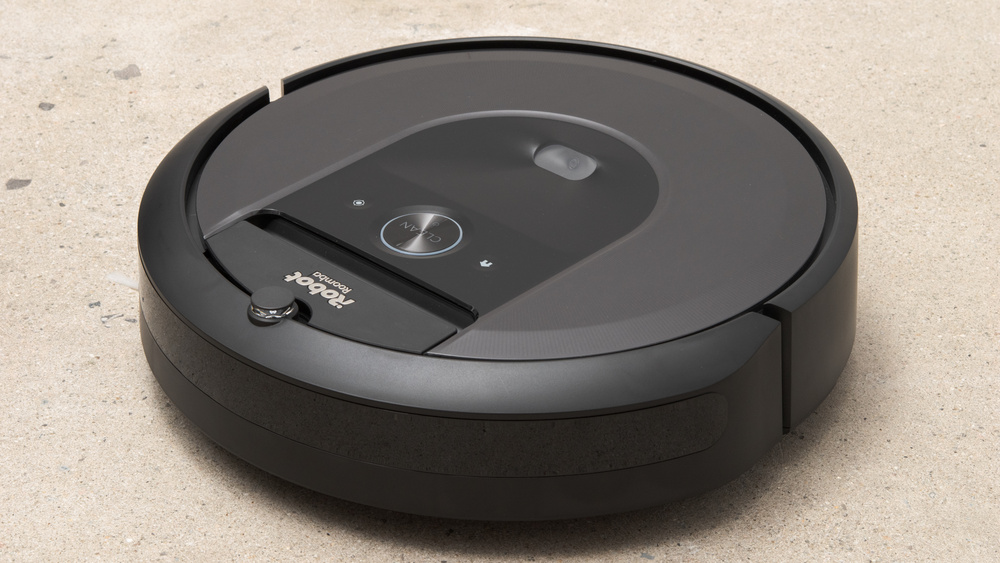
\includegraphics[width=67mm, keepaspectratio]{figures/iRobot_roomba_i7.jpg}\\\vspace{5mm}
	\caption{iRobot Roomba 780 (left) and i7 (right) (sources: \cite{roomba780}\cite{roombai7})}
	\label{fig:Roombas}
\end{figure}

With this little example we reviewed the advantages of SLAM (Simultaneous localization and mapping) in a housekeeping environment. Mobile robots and SLAM can be used in various industrial environments, too. For example, autonomous robots can carry heavy products from one place to another in a huge warehouse. In these cases it is unimaginable that a wall-to-wall algorithm could achieve a proper navigation (it is questionable if it would even arrive to its goal before draining its battery). All in all, nowadays it is very important to use some SLAM algorithm.

\section{Goal of the thesis}

The aim of this thesis is to further develop the navigation and exploration capabilities of a mobile robot, so that it can independently explore its surroundings when it arrives at a new location and create a map. This map could be reused by it or other robots.

The main goal is to use V-SLAM (Visual-SLAM) with a stereo camera instead of SLAM with a LIDAR. The reasons behind this choice are:
\begin{itemize}
    \item a camera can easily build 3D maps or point clouds of the robots' surroundings,
    \item if the camera has RGB lenses than we can create colorful point clouds of its environment,
    \item the camera can be used to detect specific objects.
\end{itemize}
One of our goals was to detect persons with the camera and prepare the robot to be able to follow or avoid them.

\section{Structure of the thesis}

TODO
